% Docummentation:
% - https://www.latex-project.org/help/documentation/
% - https://docs.w3cub.com/latex/
% - https://tex.stackexchange.com/questions/455993/formatting-sql-code
% - https://www.overleaf.com/learn/latex/Code_listing#Code_styles_and_colours

%--------------------------------------------------------------------------------
%-----------------------------------   TODO   ----------------------------------
%--------------------------------------------------------------------------------
% add section about icon source https://www.iconpacks.net/free-icon/money-bag-6384.html


\documentclass[a4paper,10pt, twoside]{report}

\usepackage{polski}         % Polish diacretic signs
\usepackage[utf8]{inputenc} % required for international characters
\usepackage{hyperref}       % urls and hyperlinks
\usepackage{xurl}           % break urls
\usepackage{microtype}      % improve justification
\usepackage{enumitem}       % compact lists
\usepackage{graphicx}       % Include graphics
\usepackage{wrapfig}        % wrap text aroung graphics
\usepackage{fancyhdr}       % Customize page layout
\usepackage{index}          % Create an index
\usepackage{setspace}       % Spacing
\usepackage{float}          % Forcing figure placement
\usepackage{tabularray}     % Tables with wrapping
\usepackage{xcolor,listings}% Code listings
\usepackage{textcomp}       % Code listings
\usepackage{color}          % Code listings
\usepackage{nameref}        % Reference chapter, section, etc. by name
\usepackage{afterpage}
\usepackage{tcolorbox}      % Colored boxes for inline Code

\makeindex
\graphicspath{ {./} }       %Was ./figures/ changed so i can peek in VS Code
%Widow and orphan control as per https://tex.stackexchange.com/questions/4152/how-do-i-prevent-widow-orphan-lines/4167#4167?newreg=87e476a8b11e44e2bd285df0190a69e0
\widowpenalty10000          
\clubpenalty10000

% Code listings
\definecolor{codegreen}{rgb}{0,0.6,0}
\definecolor{codegray}{rgb}{0.5,0.5,0.5}
\definecolor{codepurple}{HTML}{C42043}
\definecolor{backcolour}{HTML}{F2F2F2}
\definecolor{bookColor}{cmyk}{0,0,0,0.90}  
\color{bookColor}

\lstset{upquote=true}

\lstdefinestyle{mystyle}{
    backgroundcolor=\color{backcolour},   
    commentstyle=\color{codegreen},
    keywordstyle=\color{codepurple},
    numberstyle=\numberstyle,
    stringstyle=\color{codepurple},
    basicstyle=\footnotesize\ttfamily,
    breakatwhitespace=false,
    breaklines=true,
    captionpos=b,
    keepspaces=true,
    numbers=left,
    numbersep=10pt,
    showspaces=false,
    showstringspaces=false,
    showtabs=false,
}
\lstset{style=mystyle}

% Code listings
\newcommand\numberstyle[1]{%
    \footnotesize
    \color{codegray}%
    \ttfamily
    \ifnum#1<10 0\fi#1 |%
}

\renewcommand{\lstlistlistingname}{Listingi}

% ------------------------------ Custom Commands ------------------------------
% Usage: \command\{text}  
\newcommand{\customstyletitle}[1]{\Huge{\textbf{#1}}}
\newcommand{\customstylechapter}[1]{\large{\textit{#1}}}
\newcommand{\customstylesection}[1]{\textbf{\textit{#1}}}
\newcommand{\customstylesidenote}[1]{\Small{\textbf{#1}}}
\newcommand{\customstyletable}[1]{\footnotesize{\textbf{#1}}}
\newcommand{\customstyletablecentered}[1]{\footnotesize\centering{\textbf{#1}}}
\newcommand{\customstyleindivisible}[1]{
    \begin{minipage}{\textwidth}
        {#1}
    \end{minipage}
}

\lstnewenvironment{SQLlisting}[2][]%
  {\noindent\minipage{\linewidth}\medskip
   {#2}
   \smallskip
   \lstset{basicstyle=\ttfamily\footnotesize,
            frame=single,
            language=SQL,
            deletekeywords={IDENTITY},
            %deletekeywords={[2]INT},
            morekeywords={clustered},
            framesep=8pt,
            xleftmargin=40pt,
            framexleftmargin=40pt,
            frame=tb,
            framerule=0pt,
            caption=#1}}
  {\endminipage}

  % spacer
\newcommand{\HRule}{\rule{\linewidth}{0.5mm}} % horizontal lines

\newtcbox{\inlinecode}{on line, boxrule=0pt, boxsep=0pt, top=2pt, left=2pt, bottom=2pt, right=2pt, colback=gray!15, colframe=white, fontupper={\ttfamily \footnotesize}}

% --------------------------- documment starts here ---------------------------

% environment
\begin{document}

% Define pagestyle
% [REQUIREMENT] 23. Przypisy dolne, stopki (nr stron), nagłówki...
\pagestyle{fancy}
\fancyhf{}          %clears default headers and footers
\renewcommand{\headrulewidth}{2pt}
\renewcommand{\footrulewidth}{1pt}

\fancypagestyle{mychapterpage}{%
    %\fancyhead[LE]{\leftmark}
    %\fancyhead[RO]{\rightmark}
    \fancyfoot[RO,LE]{\thepage}
    \renewcommand{\headrulewidth}{2pt}
    \renewcommand{\footrulewidth}{1pt}
}


% https://texblog.org/2013/09/16/multiple-page-styles-with-fancyhdr/
%Redefine chapter by adding fancy as the chapter title page page-style
\makeatletter
    \let\stdchapter\chapter
    \renewcommand*\chapter{%
    \@ifstar{\starchapter}{\@dblarg\nostarchapter}}
    \newcommand*\starchapter[1]{%
        \stdchapter*{#1}
        \thispagestyle{mychapterpage}
        \fancyfoot[RO,LE]{\thepage}
        \markboth{\MakeUppercase{#1}}{}
    }
    \def\nostarchapter[#1]#2{%
        \stdchapter[{#1}]{#2}
        \thispagestyle{mychapterpage}
        \fancyfoot[RO,LE]{\thepage}
    }
\makeatother


% [REQUIREMENT] 1. Strona tytułowa
\begin{titlepage}
	%---Headings------------------------------------------	
	\begin{center}
    \begin{onehalfspace}
    \textsc{\LARGE{WYŻSZA SZKOŁA TECHNOLOGII INFORMATYCZNYCH W KATOWICACH}}\\
    \end{onehalfspace}
    \textsc{\large{WYDZIAŁ INFORMATYKI}}\\
	\textsc{\large{KIERUNEK: INFORMATYKA}}\\
    \end{center}
    
    %---Author--------------------------------------------
	\begin{flushleft}
    \textsc{Nowak Marcin}\\[0cm]
    \textsc{Nr Albumu 08255}\\[0cm]
    \textsc{Studia niestacjonarne}\\[0cm]
    \end{flushleft}
	
    %---Title---------------------------------------------
	\begin{center}
    \HRule\\[0.4cm]
	{\customstyletitle{Projekt i implementacja aplikacji wspomagającej zarządzanie budżetem domowym}}\\[0.4cm] 
    \HRule\\[1.5cm]
    \end{center}
	
    %---Description----------------------------------------
	\begin{flushright}
        \textsc{Przedmiot: Projekt Systemu Informatycznego}\\[0cm]
        \textsc{pod kierunkiem}\\[0cm]
        \textsc{mgr. Jacek Żywczok}\\[0cm]
        \textsc{W roku akademickim 2022/23}\\[0cm]
    \end{flushright}
 
	%---Date & logo---------------------------------------
	\vfill                  % Position the date lower
	\begin{center}
    {Katowice 2022}\\	    % \today
	
\includegraphics[width=0.2\textwidth]{figures/WSTI-logo.jpg}\\[1cm]
	\end{center}
\end{titlepage}

\null\newpage % #TODO: fix, this moves formatting \addtocounter{page}{-1}

% [REQUIREMENT] 2. Spis treści
\renewcommand*\contentsname{Spis treści}
\tableofcontents                    % prints automatical table of contents

% ---------------------------------- Content ----------------------------------


% 3.1. Wstęp <-[Wprowadzenie do tematyki projektu, Zamierzony cel projektu]
%http://siminskionline.pl/seminarium-inzynierskie/struktura-pracy-inzynierskiej/wstep/

\chapter{\customstylechapter{Wstęp}}
{Finanse są dziedziną nauki ekonomicznej któa zajmuje się rozporządzaniem 
pieniędzmi \cite{wiki_ekonomia}. Nauka ta w podobnym zakresie a różnej skali 
dotyczy państw, przedsiębiorstw jak i zwykłych obywateli - w efekcie jest to 
dziedzina o stosunkowo prostych podstawach jednak niesamowicie skomplikowana w 
każdym zakresie w którym można ją zagłębić. Wiedza z zakresu finansów staje się 
szczególnie przydatna gdy na rynku panuje trudna sytuacja ekonomiczna, w takich 
warunkach nierzadko decyduje ona o jakości oraz stanie życia poszczególnych 
osób fizycznych, rentowności przedsiębiorstw czy stabilności państw. W przypadku
 państw i firm przeważnie budżetem zarządzają dedykowane osoby lub też całe 
zespoły, posiadające ekspercką wiedzę w tej dziedzinie. Jednak osoby 
zarządzające budżetem domowym najczęściej dysponują wyłacznie nabytym 
doświadczeniem i na ogół stosują podejście intuicyjne, rzadko jeśli wogóle 
wspomagając się jakimikolwiek narzędziami które ułatwiałyby to zadanie. Wiele 
osób sposzukuje pożytecznych treści o tematyce finansowej w Internecie, jednakże 
rozpoczynając zaznajamianie się z tematyką mogą mieć spore trudność z 
odnalezieniem treści dobrej jakości w natłoku materiałów błędnych, słabych 
merytorycznie, niekatualnych czy też nastawionych na marketing ponad poprawność 
oraz przystępnością treści źródeł dobrej jakości.}

{Celem pracy jest zaprojektowanie i realizacja modułu analitycznego aplikacji 
która ułatwi jej użytkownikom zarządzanie budżetem domowym dostarczając 
narzędzia do analizy wpływów i wydatków, wizualizacji trendów oraz automatycznie 
kategoryzujące wpływy i wydatki. Będzie to aplikacja przeglądarkowa napisana w 
języku Python, wykorzystująca frameworki: frontend Bootstrap\cite{Bootstrap}, 
Flask\cite{Flask}, WTForms\cite{WTForms}, silnik szablonów jinja\cite{jinja}, 
oraz bibliotekę chart.js\cite{chart.js} do generowania wizualizacji.}

% #TODO: Dodaj łamanie
% #TODO: Uzupełniać w trakcie "Streszczenie zawartości kolejnych rozdziałów (...) Ten fragment to zakres pracy."
{Rozdział drugi zawiera rozwinięcie charakterystyki i motywacji problemu krótko 
zaznaczonej we wstępie pracy. Rozdział trzeci to analiza istniejących rozwiązań.}

% 3.2. Charakterystyka/analiza problemu
%http://siminskionline.pl/seminarium-inzynierskie/struktura-pracy-inzynierskiej/charakterystykaanaliza-problemu/
\chapter{\customstylechapter{Charakterystyka i analiza problemu}}

{Na dzień dzisiejszy wiedza z zakresu finansów oferowana w ramach systemu 
edukacji publicznej jest znikoma\cite{edukacjafinansowawszkołach}. Sytuacja ta 
ma miejsce od dawna, dlatego spora część obywateli Polski słabo orientuje się w 
kwestii finansów osobistych, ekonomii i przedsiębiorczości. Istnieje wiele 
aktywnie działających programów które wprowadzają uczestników w świat finansów 
poprzez przedstawienie podstawowych zagadnień z dziedziny ekonomii i podstaw 
inwestowania\cite{edukacjafinansowawszkołach}. Działania te mają na celu 
zbudować w nich świadomość ogólnej sytuacji ekonomicznej jednakże jak wynika z 
badań Banku Pekao\cite{edukacjafinansowamlodziezy}, większość rodziców stwierdza
 że nie posiada wystarczającej wiedzy o finansach żeby przekazać ją dzieciom, 
co pozwala wysnuć wniosek iż sami zarządzają finansami rodzinnymi korzystając 
raczej z intuicji i własnego doświadczenia aniżeli solidnych podstaw 
teretycznych. Tego rodzaju podejście na wyczucie, przez większość czasu działa. 
Wydaje się że nie ma większego wpływu na życie gdy sytuacja ekonomiczna jest 
spokojna - zmiana podejścia pozwala wtedy co prawda więcej zaoszczędzić, jednak 
w zasadzie jest to opcjonalne. Kiedy jednak na rynku czy to lokalnym czy 
globalnym pojawiają się zawirowania które powodują nagły wzrost inflacji 
przeważnie koszta życia rosną niewspółmiernie do 
zarobków\cite{gussytuacjabudzetowa}, a tym samym dopięcie finansów osobistych i 
domowych tak, by bilans wyszedł dodatni wymaga więcej uwagi. W ostatnich latach 
miało miejsce kilka tego typu zdarzeń któe dotknęły światową ekonomię. W 
momencie pisania tej pracy takimi wydarzeniami są pandemia Covid 19 oraz agresja
 Rosji na Ukrainę. Zdarzenia te jak wynika z badań Krajowego Rejestru Długów 
\cite{portfelpolakawpandemii} u prawie połowy polaków wywołała poczucie 
zagrożenia biedą, podczas gdy jedynie 22\% twierdzi że jest spokojna o swoją 
sytuację finansową. Raport Warsaw Enterprise Institute \cite{weiinflacja} 
wykazuje natomiast spadek realnych płac (uwzględniających zarobki oraz wydatki) 
średnio o 2\%, a w niektórych grupach możliwe 5-11\% w latach 2020-2022.}

\begin{figure}[H]           %requires float package
    \caption{Główny Urząd Statystyczny, Dynamika realnych dochodów i wydatków na 1 osobę w gospodarstwach domowych
    w latach 2010–2022\cite{gussytuacjabudzetowa}}
    \label{fig:}
    \centering  
    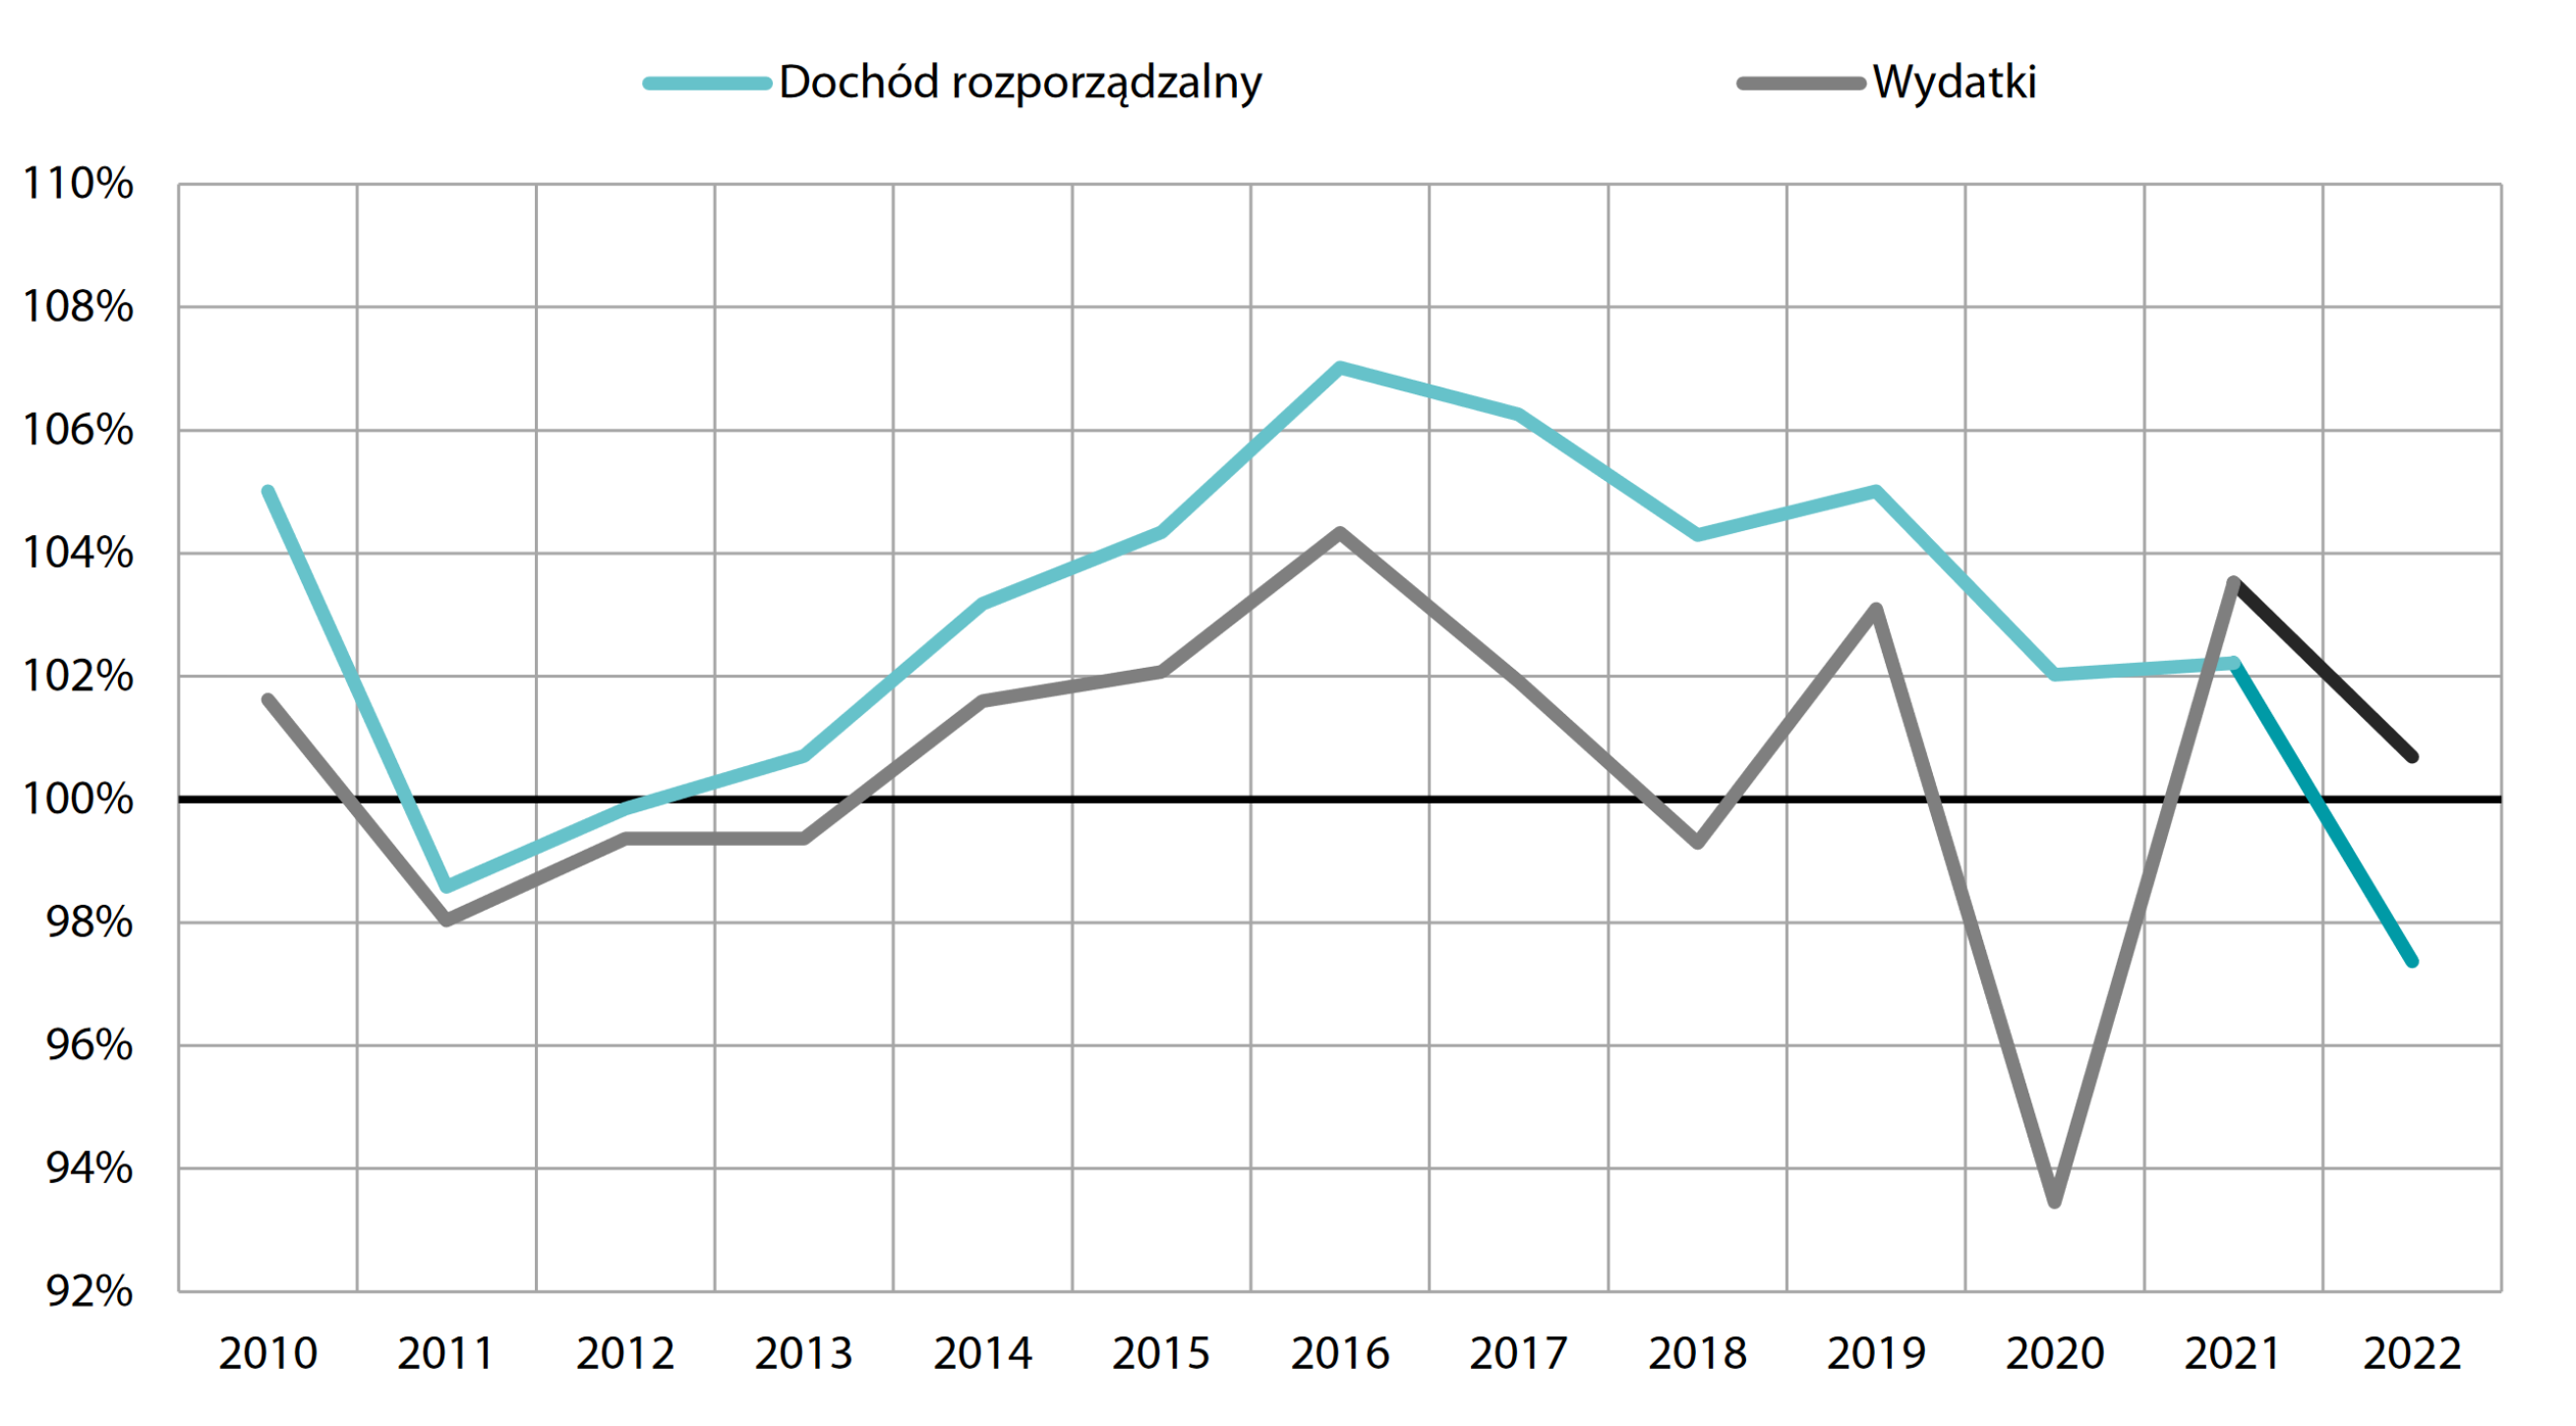
\includegraphics[width=12cm]{figures/GUS_dynamikarealnychdochodowiwydatkow2010-2020.png}
\end{figure}

\begin{figure}[H]           %requires float package
    \caption{300gospodarka.p, Inflacja w Polsce w latach 1996-2023 dane GUS}
    \label{fig:}
    \centering  
    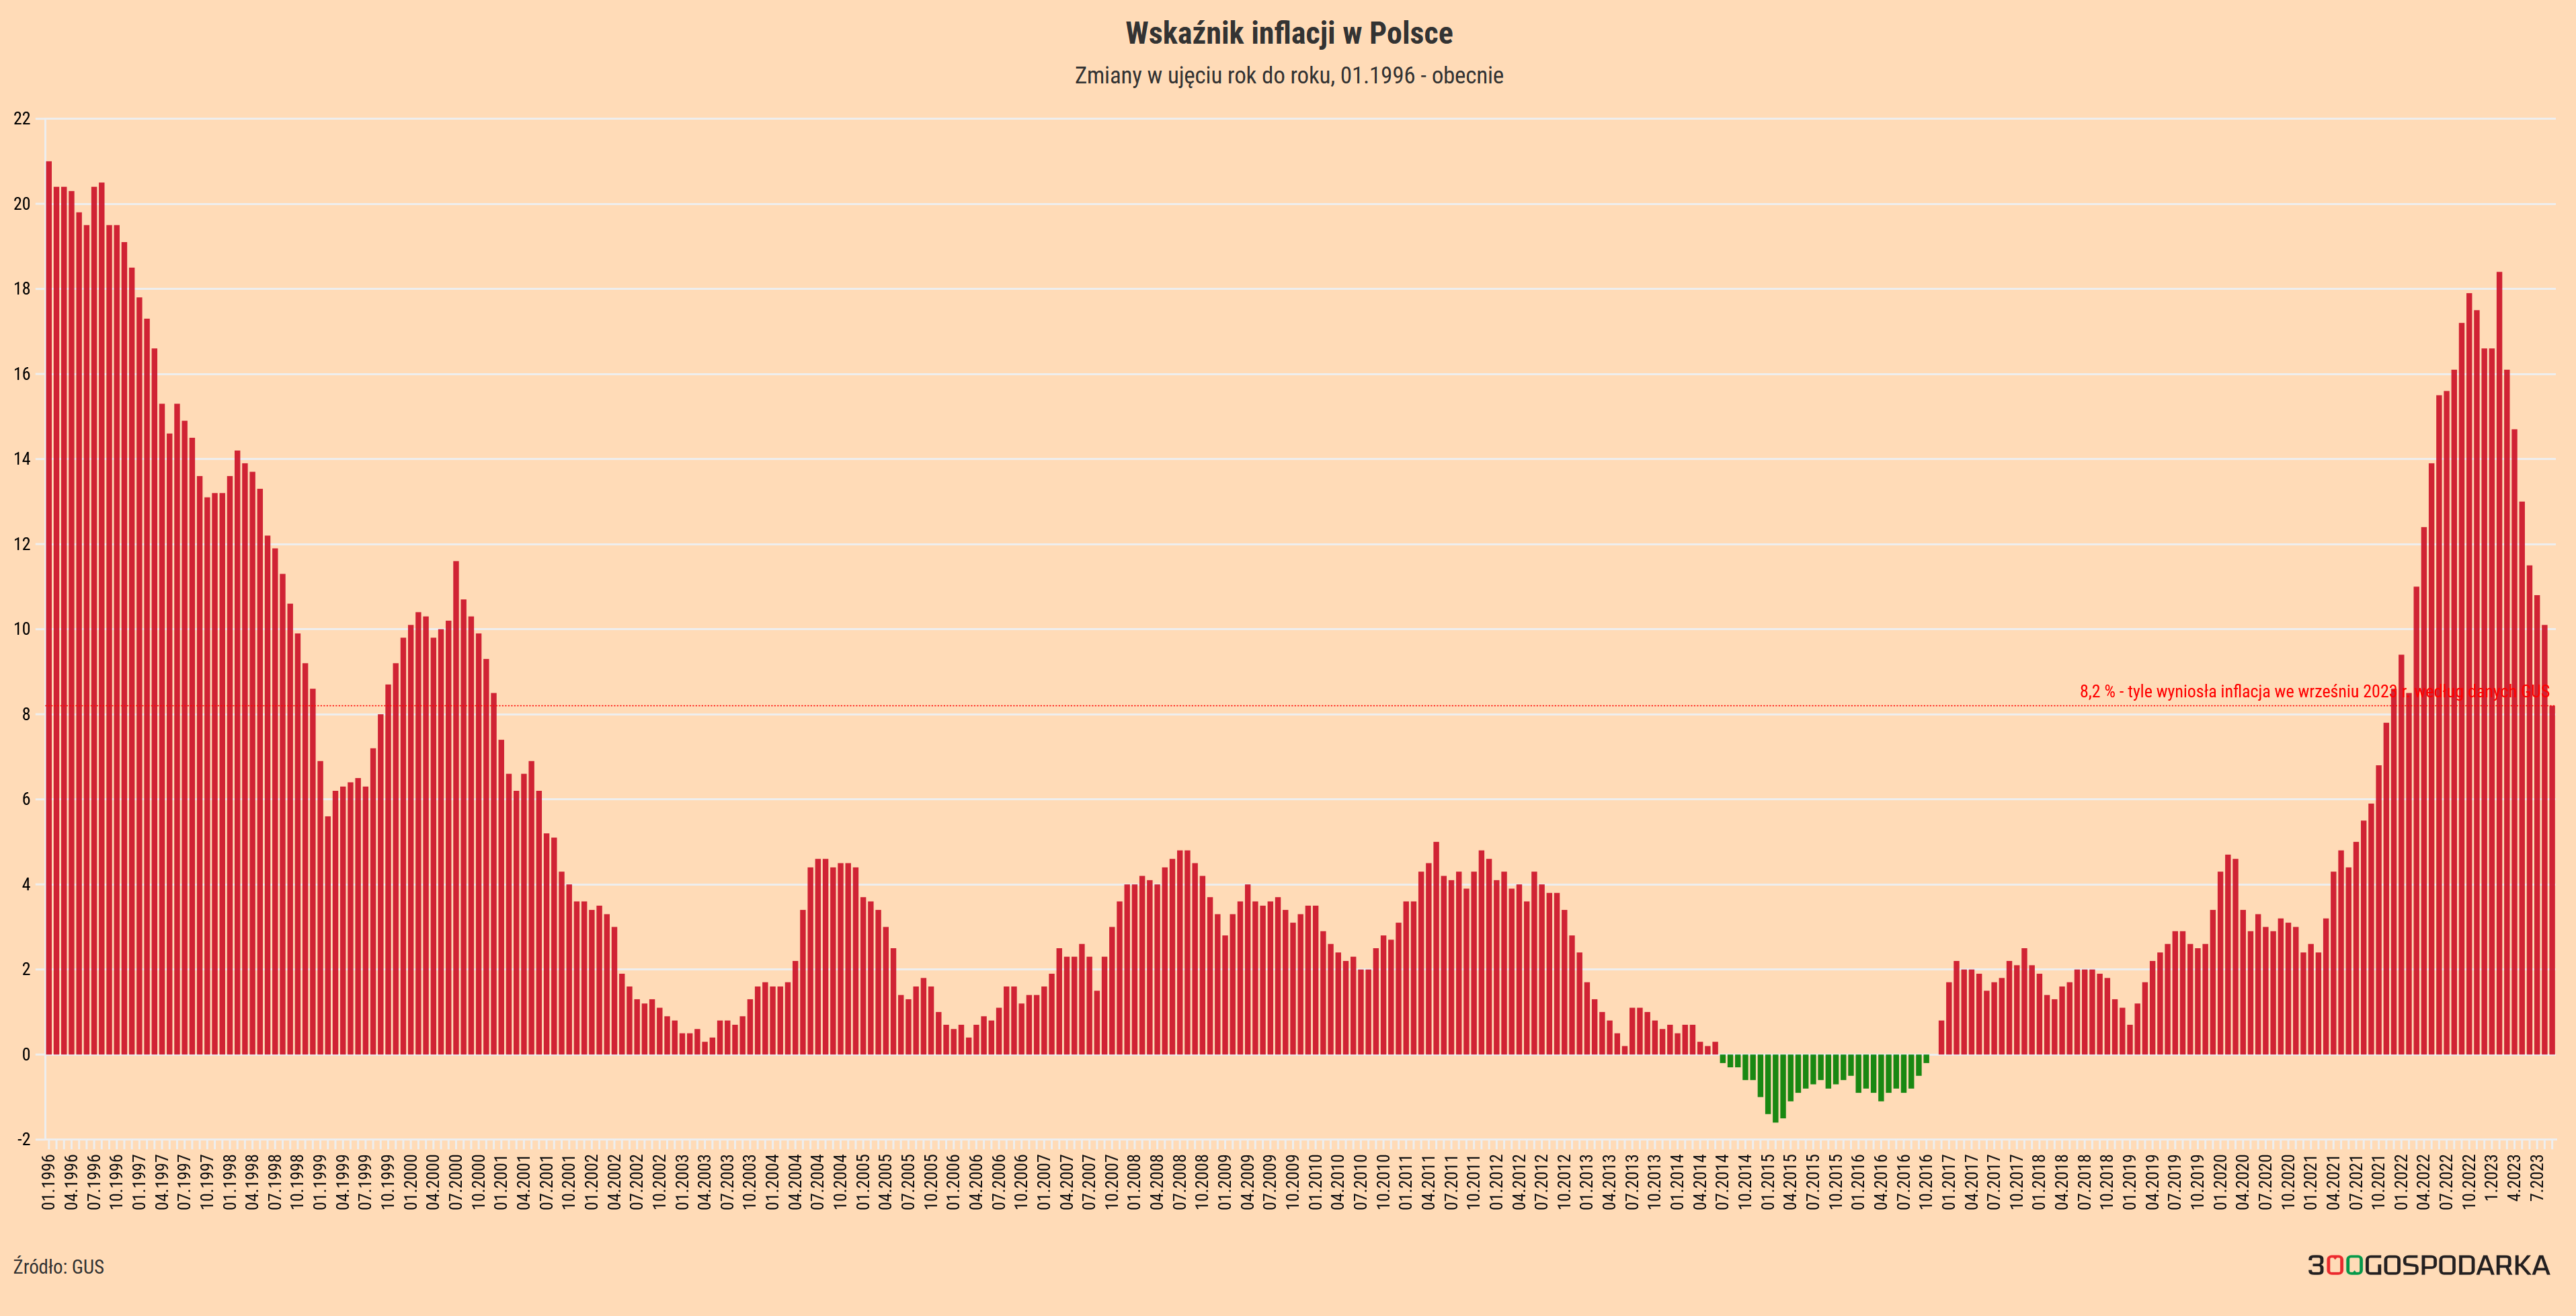
\includegraphics[width=12cm]{figures/300gospodarka-pl_inflacjawpolsce.png}
\end{figure}


{Podstawowym narzędziem które może pomóc utrzymać wydatki na odpowiednim 
poziomie jest planowanie domowego budżetu. Wymaga to dwóch etapów - po pierwsze 
metody lub narzędzia które ułatwią zarządzanie budżetem domowym oraz znajomości 
podstaw zarządzania finansami. Dlatego dla osób rozpoczynających budżetowanie 
ważne jest przedstawienie w możliwie prostej, zwięzłej i przystępnej formie już 
gotowych opracowanych rozwiązań które można zastosować aby świadomie zarządzać 
sytuacją finansową własnego domostwa. W najprostszym wariancie na 
budżet\cite{o24_budzetowanie}\cite{budget}\cite{mintbudget} składają się: 
wpływy czyli dochody ze wszystkich źródeł, zobowiązania czyli płatności stałe 
jak rachunki czy raty kredytów oraz wydatki które są zróżnicowane. Skrupulatne 
zbieranie danych z pewnego okresu pozwala dostrzec ogólną sytuację finansową, a 
w miarę jak zakres czasu dostępnych danych się wydłuża a ich precyzja zwiększa 
pojawia się także możliwość wysłuskania trendu przez co i prognozowania 
przyszłej sytuacji. Istnieje wiele różnych podejść do tworzenia budżetu - od 
najbardziej ogólnych które skupiają się wyłącznie na określeniu bilansu wydatków
 oraz wpływów, po najbardziej szczegółowe analizy wydatków na poszczególne 
kategorie czy nawet produkty. Każde z podejść ma swoje dobre strony, i w gruncie
 rzeczy każdy powinien wybrać podejście odpowiednie dla siebie.}


\begin{figure}[H]           %requires float package
    \caption{oszczedzaniepieniedzyblog.pl, Najprostszy budżet - przychody}
    \label{fig:}
    \centering  
    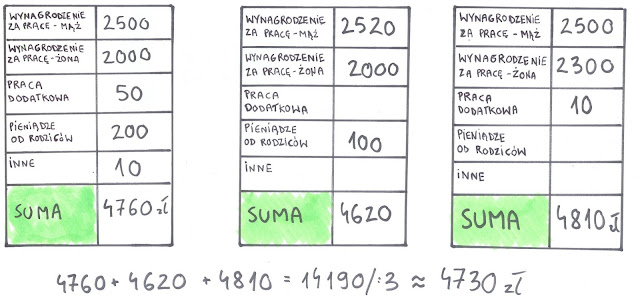
\includegraphics[width=12cm]{figures/oszczedzaniepieniedzyblog-pl_przychody.jpg}
\end{figure}


\begin{figure}[H]           %requires float package
    \caption{oszczedzaniepieniedzyblog.pl, Najprostszy budżet - wydatki}
    \label{fig:}
    \centering  
    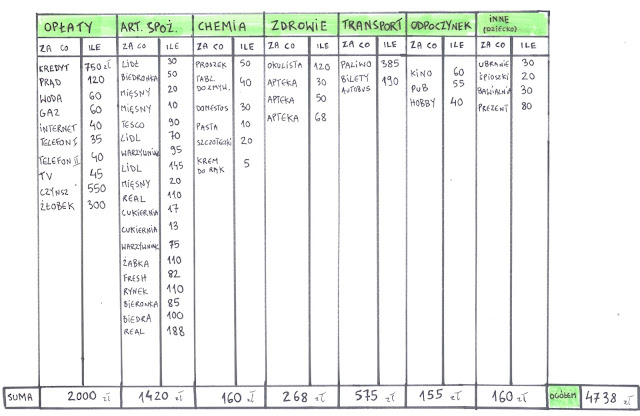
\includegraphics[width=12cm]{figures/oszczedzaniepieniedzyblog-pl_wydatki.jpg}
\end{figure}


{Poza ukazaniem ogólnego obrazu sytuacji budżetowej w budżecie uwzględnić można 
cele jak spłata zadłużenia, czy planowany znaczny wydatek, oraz limity 
pomagające ograniczyć wydatki i cele przychodów zwiększające ilość dostępnych 
środków finansowych. W literaturze przedmiotowej opisano także wiele przydatnych
 podejść oraz zasad jak wstępny podział wydatków na podstawie 
priorytetów\cite{najbogatszyczlowiekwbabilonie} czy uwzględnienie oszczędzania 
w formie najpierw zapłać sobie\cite{najbogatszyczlowiekwbabilonie}
\cite{finansowaforteca} które można zastosować jako strategie zarządzania 
finansami domowymi aby poprawić sytuację finansową lub osiągnąć zamierzony cel. 
Jednak aby zastosować daną strategię trzeba ją najpierw znać, a jak opisano 
wcześniej poziom wiedzy z zakresu finansó w Polsce jest słaby, dlatego narzędzia
 do zarządzania finansami powinny w najprostszej formie udostępniać takie 
informacje w łatwo przystępnej formie, a idealnie posiadać zabudowane mechanizmy
 które pozwoliłyby użytkownikowi wybrać i zastosować strategię bez potrzeby jej 
dogłębnej znajomości.}

{Z uwagi na tematykę z zasady są to dane bardzo wrażliwe, zatem muszą być 
odpowiednio zabezpieczone. Idealną opcją dla potencjalnych użytkowników byłoby 
gdyby jako jedyni mieli dostęp do prywatnych danych, lub mogli je współdzielić 
z wybranymi przez siebie osobami. Przy znaczącej statystycznie ilości 
użytkowników dane zebrane w aplikacji po odpowiedniej anonimizacji i 
uśrednieniu mogą posłużyć do modelowania wydatków obywateli danych regionów, 
sektorów, segmentów gospodarki lub nawet ogólnie całego państwa, co z kolei 
można wykorzystać zwrotnie w samej aplikacji aby porównać model wydatków 
użytkownika do adekwatnej średniej i zwrócić uwagę na obszary w których 
pozytywnie od niej odstaje co moze zaowocować pozytywnym wzmocnieniem dobrego 
nawyku a nawet chęcią dalszej poprawy w innej kategorii wydatków. Tego typu 
modelowanie jest już przeprowadzane przez Główny Urząd Statystyczny, którego 
raporty publikowane są co roku, jest to więc potencjalne najlepsze źródło 
najlepszych danych, które mogłoby zostać wykorzystane do porównań.}


% #TODO: Continue from here
% 3.3. Analiza istniejących rozwiązań


% [#TODO]:
% 3.3. Analiza istniejących rozwiązań
% 3.4. Koncepcja własnego rozwiązania
% 3.5. Projekt ogólny
% 3.6. Dokumentacja techniczna
% 3.7. Testy i weryfikacja systemu
% 3.8. Przykładowy scenariusz wykorzystania systemu
% 3.9. Zakończenie
% 3.13.Ewentualne załączniki


% #TODO: Remove unused sources
% 3.10.Bibliografia
\begin{thebibliography} {books}
    \bibitem{najbogatszyczlowiekwbabilonie} George S. Clason, (2021) Najbogatszy człowiek w Babilonie, ISBN: 978-83-67060-04-2
    \bibitem{finansowaforteca} Marcin Iwuć, (2020) Finansowa Forteca, ISBN: 978-83-958468-0-9
    \bibitem{wiki_ekonomia} Wikipedia, Nauki Ekonomiczne \raggedright\url{
        https://pl.wikipedia.org/wiki/Nauki_ekonomiczne}
    \bibitem{gussytuacjabudzetowa} Główny Urząd Statystyczny, Budżety gospodarstw domowych w 2022 roku \raggedright\url{
        https://stat.gov.pl/obszary-tematyczne/warunki-zycia/dochody-wydatki-i-warunki-zycia-ludnosci/budzety-gospodarstw-domowych-w-2022-roku,9,21.html}
    \bibitem{o24_budzetowanie} Opcje24, Budzetowanie \raggedright\url{
        https://www.opcje24h.pl/budzetowanie-przewodnik-planowanie-budzetu/}
    \bibitem{MOSCOW} Product Plan, MOSCOW Prioritetization \raggedright\url{
        https://www.productplan.com/glossary/moscow-prioritization/}
    \bibitem{MatrycaEisenhowera}Praca.pl, Matryca Eisenhowera - czym jest, zasada, prioryteryzacja zadań \raggedright\url{
        https://www.praca.pl/poradniki/rynek-pracy/matryca-eisenhowera-czym-jest,zasada,prioryteryzacja-zadan_pr-2012.html}
    \bibitem{MVP} Wikipedia, Minimal Viable Product \raggedright\url{
        https://en.wikipedia.org/wiki/Minimum_viable_product}
    \bibitem{ISO 8601} NASA.gov, A summary of the international standard date and time notation \raggedright\url{
        https://fits.gsfc.nasa.gov/iso-time.html}
    \bibitem{CSV} Y. Shafranovich, SolidMatrix Technologies, Inc., Common Format and MIME Type for Comma-Separated Values (CSV) Files \raggedright\url{
        https://www.rfc-editor.org/rfc/rfc4180}
    \bibitem{SQLite} sqlite.org, SQLite \raggedright\url{
        https://www.sqlite.org/index.html}
    \bibitem{SQL} wikipedia.org, SQL - Structured Query Language \raggedright\url{
        https://en.wikipedia.org/wiki/SQL}
    \bibitem{Python} python.org, Python \raggedright\url{
        https://www.python.org/}
    \bibitem{PySimpleGUI} pysimplegui.org, PySimpleGUI Python GUIs for Humans \raggedright\url{
        https://www.pysimplegui.org/en/latest/}
    \bibitem{JSON} json.org, Introducing JSON \raggedright\url{
        https://www.json.org/json-en.html}
    \bibitem{Python_read-file} pythonspot.com, Python tutorials, How to Read a File in Python \raggedright\url{
        https://pythonspot.com/read-file/}
    \bibitem{Trello} Atlassian, Trello.com \raggedright\url{
        https://trello.com/}
    \bibitem{StarUML} MKLabs Co.,Ltd, StarUML \raggedright\url{
        https://staruml.io/}
    \bibitem{LaTeX} The LaTeX Project \raggedright\url{
        https://www.latex-project.org/}
    \bibitem{VSCode} Microsoft, Visual Studio Code \raggedright\url{
        https://code.visualstudio.com/}
    \bibitem{DataGrid} JetBrains, DataGrid \raggedright\url{
        https://www.jetbrains.com/datagrip/}
    \bibitem{Kanban} Lean Action PLan, Kanban – układ nerwowy sterowania produkcją w koncepcji Lean Manufacturing \raggedright\url{
        https://leanactionplan.pl/kanban/}
    \bibitem{LEAN} Wikipedia, Lean software development \raggedright\url{
        https://pl.wikipedia.org/wiki/Lean_software_development}
    \bibitem{GIT} git-scm.com, git \raggedright\url{
        https://git-scm.com/}
    \bibitem{GitHub} https://github.com/ \raggedright\url{
        https://github.com/}
    \bibitem{Model Przyrostowy} Wikipedia, Model Przyrostowy \raggedright\url{
        https://pl.wikipedia.org/wiki/Model_przyrostowy}
    \bibitem{EdittableTable} YouTube The CS Classroom, PySimpleGUI - Excel-style Editable Table \raggedright\url{
        https://www.youtube.com/watch?v=ETHtvd-_FJg}
    \bibitem{Tkinter} python.org, tkinter — Python interface to Tcl/Tk \raggedright\url{
        https://docs.python.org/3/library/tkinter.html}
    \bibitem{PyInstaller} pyinstaller.org, PyInstaller Manual \raggedright\url{
        https://pyinstaller.org/en/stable/}
    \bibitem{GITBudgeterApp} github.com MarcinNowak94, DatabaseShenanigans \raggedright\url{
        https://github.com/MarcinNowak94/DatabaseShenanigans}
    \bibitem{GITBudgeterDoc} github.com MarcinNowak94, budgeter \raggedright\url{
        https://github.com/MarcinNowak94/budgeter}
    \bibitem{GITRighten} github.com MarcinNowak94, Righten \raggedright\url{
        https://github.com/MarcinNowak94/Righten}
    \bibitem{Bootstrap} getbootstrap.com, Bootstrap \raggedright\url{
        https://getbootstrap.com/}
    \bibitem{Flask} flask.palletsprojects.com, Flask \raggedright\url{
        https://flask.palletsprojects.com/en/3.0.x/}
    \bibitem{WTForms} wtforms.readthedocs.io, WTForms \raggedright\url{
        https://wtforms.readthedocs.io/en/3.1.x/}
    \bibitem{jinja} jinja.palletsprojects.com, Jinja \raggedright\url{
        https://jinja.palletsprojects.com/en/3.1.x/}
    \bibitem{chart.js} www.chartjs.org, Chart.js \raggedright\url{
        https://www.chartjs.org/}
    \bibitem{edukacjafinansowawszkołach} Łukasz Grygiel, Jak wygląda edukacja finansowa dzieci i młodzieży w Polsce? \raggedright\url{
        https://web.archive.org/web/20230529115945/https://lukaszgrygiel.com/edukacja-finansowa-dzieci-i-mlodziezy/}
    \bibitem{edukacjafinansowamlodziezy} Bank Pekao, Raport Banku Pekao: „Dziecięcy świat finansów - jak rynek finansowy odpowiada na potrzeby najmłodszych klientów”. \raggedright\url{
        https://www.pekao.com.pl/o-banku/aktualnosci/d4e423aa-0ba4-4bde-8a0a-7ff3a17a9793/raport-banku-pekao-dzieciecy-swiat-finansow-jak-rynek-finansowy-odpowiada-na-potrzeby-najmodszych-klientow.html}
    \bibitem{portfelpolakawpandemii} Krajowy Rejestr Długów, Portfel statystycznego Polaka w pandemii \raggedright\url{
        https://krd.pl/centrum-prasowe/raporty/2022/portfel-statystycznego-polaka-w-pandemii}
    \bibitem{budget} The Balance, Understanding Budgeting \& Personal Finance\raggedright\url{
        https://www.thebalancemoney.com/personal-finance-budget-4802696}
    \bibitem{mintbudget} www.mint.intuit.com, Budgeting 101 \raggedright\url{
        https://mint.intuit.com/blog/category/budgeting/}
    \bibitem{koszty2010-22} Warsaw Enterprise Institute, [RAPORT] Żegnajcie niskie ceny? Koszty życia i poziom cen w Polsce na tle krajów UE w latach 2010–2022 \raggedright\url{
        https://wei.org.pl/2022/aktualnosci/wiktorwojciechowski/raport-zegnajcie-niskie-ceny-koszty-zycia-i-poziom-cen-w-polsce-na-tle-krajow-ue-w-latach-2010-2022/}
    \bibitem{weiinflacja} Warsaw Enterprise Institute, [RAPORT] Jak inflacja zubaża Polaków? \raggedright\url{
        https://wei.org.pl/2023/publikacje/raporty/mateusz-benedyk/raport-jak-inflacja-zubaza-polakow/}
\end{thebibliography}

% 3.11.Spis rysunków
\listoffigures
% 3.12.Spis tabel
\listoftables
\lstlistoflistings

\end{document}

% Phase 2: Bachelors thesis ----------------------------------------------------
% [DONE]:
% 0. [SELF] Rename projects
% 1. [SELF] Change repository so code and docummentation are in one project
% 2. [SELF] Add Licence
% 3. [Initial review] Change structure to adhere to rules described here:
% http://siminskionline.pl/seminarium-inzynierskie/struktura-pracy-inzynierskiej/
% 3.1. Wstęp <-[sections moved here: Motywacja, cel i plan działania]
% 3.2. Charakterystyka/analiza problemu
% 3.10.Bibliografia
% 3.11.Spis rysunków
% 3.12.Spis tabel


%#TODO: rate this feature